\documentclass[pdflatex,iicol,sn-mathphys-num]{sn-jnl}

\usepackage{graphicx}
\usepackage{amsmath,amssymb,amsfonts}
\usepackage{amsthm}
\usepackage{booktabs}
\usepackage{xcolor}
\usepackage{tikz}
\usetikzlibrary{arrows.meta,positioning}

\theoremstyle{thmstyleone}
\newtheorem{theorem}{Theorem}
\newtheorem{proposition}[theorem]{Proposition}
\newenvironment{widetable}{\begin{table*}[t]}{\end{table*}}
\newenvironment{widefigure}{\begin{figure*}[t]}{\end{figure*}}

\newcommand{\AblAssistFullEightAuc}{0.6843}
\newcommand{\AblAssistFullEightRmse}{0.90}
\newcommand{\AblAssistFullOneAuc}{0.6183}
\newcommand{\AblAssistFullOneRmse}{1.68}
\newcommand{\AblAssistFullTwoAuc}{0.6335}
\newcommand{\AblAssistFullTwoRmse}{1.45}
\newcommand{\AblAssistNeitherEightAuc}{0.6300}
\newcommand{\AblAssistNeitherEightRmse}{2.00}
\newcommand{\AblAssistNeitherOneAuc}{0.5587}
\newcommand{\AblAssistNeitherOneRmse}{14.46}
\newcommand{\AblAssistNeitherTwoAuc}{0.5741}
\newcommand{\AblAssistNeitherTwoRmse}{7.38}
\newcommand{\AblAssistNoDampEightAuc}{0.6367}
\newcommand{\AblAssistNoDampEightRmse}{1.91}
\newcommand{\AblAssistNoDampOneAuc}{0.5619}
\newcommand{\AblAssistNoDampOneRmse}{14.27}
\newcommand{\AblAssistNoDampTwoAuc}{0.5775}
\newcommand{\AblAssistNoDampTwoRmse}{7.18}
\newcommand{\AblAssistNoPseudoEightAuc}{0.6584}
\newcommand{\AblAssistNoPseudoEightRmse}{1.21}
\newcommand{\AblAssistNoPseudoOneAuc}{0.5929}
\newcommand{\AblAssistNoPseudoOneRmse}{3.07}
\newcommand{\AblAssistNoPseudoTwoAuc}{0.6034}
\newcommand{\AblAssistNoPseudoTwoRmse}{2.45}
\newcommand{\AblJunyiFullEightAuc}{0.7494}
\newcommand{\AblJunyiFullEightRmse}{0.23}
\newcommand{\AblJunyiFullOneAuc}{0.7407}
\newcommand{\AblJunyiFullOneRmse}{0.57}
\newcommand{\AblJunyiFullTwoAuc}{0.7465}
\newcommand{\AblJunyiFullTwoRmse}{0.39}
\newcommand{\AblJunyiNeitherEightAuc}{0.7484}
\newcommand{\AblJunyiNeitherEightRmse}{0.70}
\newcommand{\AblJunyiNeitherOneAuc}{0.6862}
\newcommand{\AblJunyiNeitherOneRmse}{12.23}
\newcommand{\AblJunyiNeitherTwoAuc}{0.7281}
\newcommand{\AblJunyiNeitherTwoRmse}{5.13}
\newcommand{\AblJunyiNoDampEightAuc}{0.7484}
\newcommand{\AblJunyiNoDampEightRmse}{0.70}
\newcommand{\AblJunyiNoDampOneAuc}{0.6968}
\newcommand{\AblJunyiNoDampOneRmse}{12.29}
\newcommand{\AblJunyiNoDampTwoAuc}{0.7303}
\newcommand{\AblJunyiNoDampTwoRmse}{5.34}
\newcommand{\AblJunyiNoPseudoEightAuc}{0.7494}
\newcommand{\AblJunyiNoPseudoEightRmse}{0.24}
\newcommand{\AblJunyiNoPseudoOneAuc}{0.7159}
\newcommand{\AblJunyiNoPseudoOneRmse}{1.38}
\newcommand{\AblJunyiNoPseudoTwoAuc}{0.7419}
\newcommand{\AblJunyiNoPseudoTwoRmse}{0.72}
\newcommand{\AblSynTenNonFullEightAuc}{0.8010}
\newcommand{\AblSynTenNonFullEightRmse}{0.49}
\newcommand{\AblSynTenNonFullOneAuc}{0.7426}
\newcommand{\AblSynTenNonFullOneRmse}{1.15}
\newcommand{\AblSynTenNonFullTwoAuc}{0.7750}
\newcommand{\AblSynTenNonFullTwoRmse}{0.86}
\newcommand{\AblSynTenNonNeitherEightAuc}{0.7919}
\newcommand{\AblSynTenNonNeitherEightRmse}{0.92}
\newcommand{\AblSynTenNonNeitherOneAuc}{0.6250}
\newcommand{\AblSynTenNonNeitherOneRmse}{11.59}
\newcommand{\AblSynTenNonNeitherTwoAuc}{0.6859}
\newcommand{\AblSynTenNonNeitherTwoRmse}{5.23}
\newcommand{\AblSynTenNonNoDampEightAuc}{0.7960}
\newcommand{\AblSynTenNonNoDampEightRmse}{0.84}
\newcommand{\AblSynTenNonNoDampOneAuc}{0.6450}
\newcommand{\AblSynTenNonNoDampOneRmse}{11.50}
\newcommand{\AblSynTenNonNoDampTwoAuc}{0.7071}
\newcommand{\AblSynTenNonNoDampTwoRmse}{5.16}
\newcommand{\AblSynTenNonNoPseudoEightAuc}{0.7939}
\newcommand{\AblSynTenNonNoPseudoEightRmse}{0.68}
\newcommand{\AblSynTenNonNoPseudoOneAuc}{0.6677}
\newcommand{\AblSynTenNonNoPseudoOneRmse}{2.49}
\newcommand{\AblSynTenNonNoPseudoTwoAuc}{0.7202}
\newcommand{\AblSynTenNonNoPseudoTwoRmse}{1.70}
\newcommand{\AssistAccMax}{0.75}
\newcommand{\AssistAccMin}{0.37}
\newcommand{\AssistCENAuc}{0.7580}
\newcommand{\AssistCENAucMin}{0.6762}
\newcommand{\AssistCENRho}{1.000}
\newcommand{\AssistCENRmse}{0.000}
\newcommand{\AssistCNTAuc}{0.7472}
\newcommand{\AssistCNTAucMin}{0.6586}
\newcommand{\AssistCNTRho}{0.916}
\newcommand{\AssistCNTRmse}{0.343}
\newcommand{\AssistCovMax}{95}
\newcommand{\AssistCovMedian}{42}
\newcommand{\AssistCovMin}{23}
\newcommand{\AssistDPCNTEightAuc}{0.6474}
\newcommand{\AssistDPCNTEightRho}{0.158}
\newcommand{\AssistDPCNTEightRmse}{1.109}
\newcommand{\AssistDPCNTFourAuc}{0.6435}
\newcommand{\AssistDPCNTFourRho}{0.075}
\newcommand{\AssistDPCNTFourRmse}{1.072}
\newcommand{\AssistDPCNTHalfAuc}{0.6518}
\newcommand{\AssistDPCNTHalfRho}{0.011}
\newcommand{\AssistDPCNTHalfRmse}{0.997}
\newcommand{\AssistDPCNTOneAuc}{0.6499}
\newcommand{\AssistDPCNTOneRho}{0.019}
\newcommand{\AssistDPCNTOneRmse}{1.009}
\newcommand{\AssistDPCNTTwoAuc}{0.6466}
\newcommand{\AssistDPCNTTwoRho}{0.036}
\newcommand{\AssistDPCNTTwoRmse}{1.032}
\newcommand{\AssistDPFEDEightAuc}{0.6843}
\newcommand{\AssistDPFEDEightRho}{0.359}
\newcommand{\AssistDPFEDEightRmse}{0.902}
\newcommand{\AssistDPFEDFourAuc}{0.6567}
\newcommand{\AssistDPFEDFourRho}{0.218}
\newcommand{\AssistDPFEDFourRmse}{1.166}
\newcommand{\AssistDPFEDHalfAuc}{0.6098}
\newcommand{\AssistDPFEDHalfRho}{0.035}
\newcommand{\AssistDPFEDHalfRmse}{1.828}
\newcommand{\AssistDPFEDOneAuc}{0.6183}
\newcommand{\AssistDPFEDOneRho}{0.065}
\newcommand{\AssistDPFEDOneRmse}{1.677}
\newcommand{\AssistDPFEDTwoAuc}{0.6335}
\newcommand{\AssistDPFEDTwoRho}{0.121}
\newcommand{\AssistDPFEDTwoRmse}{1.448}
\newcommand{\AssistFEDAuc}{0.7580}
\newcommand{\AssistFEDAucMin}{0.6762}
\newcommand{\AssistFEDRho}{1.000}
\newcommand{\AssistFEDRmse}{0.000}
\newcommand{\AssistItems}{3,814}
\newcommand{\AssistLOCAuc}{0.7481}
\newcommand{\AssistLOCAucMin}{0.6449}
\newcommand{\AssistLOCRho}{0.376}
\newcommand{\AssistLOCRmse}{0.726}
\newcommand{\AssistNSchools}{10}
\newcommand{\AssistResp}{144,439}
\newcommand{\AssistRespPerItem}{30}
\newcommand{\AssistRespPerUser}{57}
\newcommand{\AssistUsers}{2,010}
\newcommand{\BenchConc}{16}
\newcommand{\BenchDur}{120}
\newcommand{\BenchFiveHundredBpr}{8.9}
\newcommand{\BenchFiveHundredBpt}{4,428}
\newcommand{\BenchFiveHundredErr}{0.00}
\newcommand{\BenchFiveHundredPFifty}{192}
\newcommand{\BenchFiveHundredPNinetyFive}{266}
\newcommand{\BenchFiveHundredRec}{44,447}
\newcommand{\BenchFiveHundredTx}{88.9}
\newcommand{\BenchHundredBpr}{44.3}
\newcommand{\BenchHundredBpt}{4,428}
\newcommand{\BenchHundredErr}{0.00}
\newcommand{\BenchHundredPFifty}{177}
\newcommand{\BenchHundredPNinetyFive}{242}
\newcommand{\BenchHundredRec}{9,847}
\newcommand{\BenchHundredTx}{98.5}
\newcommand{\BenchMaxErr}{0.00}
\newcommand{\BenchRecBpr}{4,405.2}
\newcommand{\BenchRecBpt}{4,405}
\newcommand{\BenchRecErr}{0.00}
\newcommand{\BenchRecPFifty}{165}
\newcommand{\BenchRecPNinetyFive}{226}
\newcommand{\BenchRecRec}{106}
\newcommand{\BenchRecTx}{106.5}
\newcommand{\BenchReps}{3}
\newcommand{\BenchSpeedup}{728}
\newcommand{\BenchTenBpr}{442.3}
\newcommand{\BenchTenBpt}{4,423}
\newcommand{\BenchTenErr}{0.00}
\newcommand{\BenchTenPFifty}{174}
\newcommand{\BenchTenPNinetyFive}{239}
\newcommand{\BenchTenRec}{1,006}
\newcommand{\BenchTenTx}{100.6}
\newcommand{\BenchThousandBpr}{4.4}
\newcommand{\BenchThousandBpt}{4,433}
\newcommand{\BenchThousandErr}{0.00}
\newcommand{\BenchThousandPFifty}{213}
\newcommand{\BenchThousandPNinetyFive}{309}
\newcommand{\BenchThousandRec}{77,494}
\newcommand{\BenchThousandTx}{77.5}
\newcommand{\BenchWarm}{15}
\newcommand{\COneAgree}{100.00}
\newcommand{\COneAllowRate}{5.9}
\newcommand{\COneBndAgree}{100.00}
\newcommand{\COneBndAllow}{109}
\newcommand{\COneBndDisagree}{0}
\newcommand{\COneBndExpired}{107}
\newcommand{\COneBndN}{2,256}
\newcommand{\COneBndPurpose}{59}
\newcommand{\COneBndRevoked}{56}
\newcommand{\COneChainBatchMs}{2629}
\newcommand{\COneChainSingleMs}{41.1}
\newcommand{\COneChainSingleP}{64.0}
\newcommand{\COneDisagree}{0}
\newcommand{\COneGrants}{164}
\newcommand{\COneN}{10,000}
\newcommand{\COneNReasons}{12}
\newcommand{\COneNegN}{12}
\newcommand{\COneNegPass}{12}
\newcommand{\COnePdpUs}{1.3}
\newcommand{\COneRevoked}{32}
\newcommand{\COneTasks}{25}
\newcommand{\CThreeClean}{1,000}
\newcommand{\CThreeDetected}{1,000}
\newcommand{\CThreeHashLarge}{20.4}
\newcommand{\CThreeHashSmall}{0.257}
\newcommand{\CThreeN}{1,000}
\newcommand{\CThreeProofLen}{10}
\newcommand{\CThreeVerifyMs}{7.0}
\newcommand{\CTwoAuthRounds}{35,280}
\newcommand{\CTwoEvents}{469}
\newcommand{\CTwoFalseDenyRound}{0}
\newcommand{\CTwoTasks}{200}
\newcommand{\CTwoViolJoin}{4,720}
\newcommand{\CTwoViolLogin}{4,720}
\newcommand{\CTwoViolRound}{0}
\newcommand{\EtoeAdmitPFifty}{1.53}
\newcommand{\EtoeAdmitPNinetyFive}{2.59}
\newcommand{\EtoeAuditDecisions}{1,049}
\newcommand{\EtoeAuditMeta}{1,049}
\newcommand{\EtoeAuditProofs}{1,049}
\newcommand{\EtoeAuditRecords}{1,049}
\newcommand{\EtoeAuditValid}{1,049}
\newcommand{\EtoeCommitMean}{2.17}
\newcommand{\EtoeExampleCommit}{2.16}
\newcommand{\EtoeExampleDenied}{1}
\newcommand{\EtoeExampleDpAfter}{0.875}
\newcommand{\EtoeExampleDpBefore}{0.916}
\newcommand{\EtoeExampleExcluded}{7}
\newcommand{\EtoeExampleFedAfter}{0.294}
\newcommand{\EtoeExampleFedBefore}{0.290}
\newcommand{\EtoeExampleFedChange}{0.251}
\newcommand{\EtoeExampleRecords}{188}
\newcommand{\EtoeExampleRound}{7}
\newcommand{\EtoeGateAfter}{2.48}
\newcommand{\EtoeGateBefore}{0.74}
\newcommand{\EtoeGateTotal}{34}
\newcommand{\EtoeOffline}{0.3}
\newcommand{\EtoeRaceExcluded}{9}
\newcommand{\EtoeRaceReason}{was invalidated at commit}
\newcommand{\EtoeRaceRound}{9}
\newcommand{\EtoeRevokeRounds}{3, 7, 11 and 15}
\newcommand{\EtoeRounds}{20}
\newcommand{\EtoeRuns}{4}
\newcommand{\EtoeTask}{35}
\newcommand{\EtoeThreeGate}{2.34}
\newcommand{\EtoeThreeTotal}{47}
\newcommand{\EtoeTxPerTask}{190}
\newcommand{\ExJunyiFedEightAuc}{0.7494}
\newcommand{\ExJunyiFedEightRmse}{0.230}
\newcommand{\ExJunyiFedFourAuc}{0.7487}
\newcommand{\ExJunyiFedFourRmse}{0.281}
\newcommand{\ExJunyiFedHalfAuc}{0.7280}
\newcommand{\ExJunyiFedHalfRmse}{0.812}
\newcommand{\ExJunyiFedOneAuc}{0.7407}
\newcommand{\ExJunyiFedOneRmse}{0.573}
\newcommand{\ExJunyiFedTwoAuc}{0.7465}
\newcommand{\ExJunyiFedTwoRmse}{0.392}
\newcommand{\ExJunyiRatioEight}{1.1}
\newcommand{\ExJunyiRatioFour}{1.3}
\newcommand{\ExJunyiRatioHalf}{1.9}
\newcommand{\ExJunyiRatioOne}{1.9}
\newcommand{\ExJunyiRatioTwo}{1.7}
\newcommand{\ExJunyiSecEightAuc}{0.7496}
\newcommand{\ExJunyiSecEightRmse}{0.206}
\newcommand{\ExJunyiSecFourAuc}{0.7496}
\newcommand{\ExJunyiSecFourRmse}{0.211}
\newcommand{\ExJunyiSecHalfAuc}{0.7454}
\newcommand{\ExJunyiSecHalfRmse}{0.438}
\newcommand{\ExJunyiSecOneAuc}{0.7484}
\newcommand{\ExJunyiSecOneRmse}{0.302}
\newcommand{\ExJunyiSecTwoAuc}{0.7493}
\newcommand{\ExJunyiSecTwoRmse}{0.233}
\newcommand{\ExRatioMax}{1.9}
\newcommand{\ExRatioMaxWhere}{Junyi, $\varepsilon=1$}
\newcommand{\ExRatioMin}{1.1}
\newcommand{\ExRatioMinWhere}{Junyi, $\varepsilon=8$}
\newcommand{\ExSeedsJunyi}{5}
\newcommand{\ExSynFedEightAuc}{0.8010}
\newcommand{\ExSynFedEightRmse}{0.489}
\newcommand{\ExSynFedFourAuc}{0.7934}
\newcommand{\ExSynFedFourRmse}{0.634}
\newcommand{\ExSynFedHalfAuc}{0.7024}
\newcommand{\ExSynFedHalfRmse}{1.446}
\newcommand{\ExSynFedOneAuc}{0.7426}
\newcommand{\ExSynFedOneRmse}{1.148}
\newcommand{\ExSynFedTwoAuc}{0.7750}
\newcommand{\ExSynFedTwoRmse}{0.861}
\newcommand{\ExSynRatioEight}{1.3}
\newcommand{\ExSynRatioFour}{1.5}
\newcommand{\ExSynRatioHalf}{1.5}
\newcommand{\ExSynRatioOne}{1.7}
\newcommand{\ExSynRatioTwo}{1.7}
\newcommand{\ExSynSecEightAuc}{0.8049}
\newcommand{\ExSynSecEightRmse}{0.372}
\newcommand{\ExSynSecFourAuc}{0.8039}
\newcommand{\ExSynSecFourRmse}{0.411}
\newcommand{\ExSynSecHalfAuc}{0.7670}
\newcommand{\ExSynSecHalfRmse}{0.957}
\newcommand{\ExSynSecOneAuc}{0.7895}
\newcommand{\ExSynSecOneRmse}{0.693}
\newcommand{\ExSynSecTwoAuc}{0.8003}
\newcommand{\ExSynSecTwoRmse}{0.509}
\newcommand{\ExtrapBatchMin}{3.5}
\newcommand{\ExtrapRecHours}{42.3}
\newcommand{\FJunyiClipCntEightPct}{96.6}
\newcommand{\FJunyiClipCntFourPct}{100.0}
\newcommand{\FJunyiGradClipHalfPct}{95.6}
\newcommand{\FJunyiGradClipTwoPct}{66.5}
\newcommand{\FJunyiSensAucMax}{0.7466}
\newcommand{\FJunyiSensAucMin}{0.7381}
\newcommand{\FJunyiSensBest}{$C=0.25$, $C_n=2$}
\newcommand{\FJunyiSensFrozenRmse}{0.393}
\newcommand{\FJunyiSensRmseMax}{0.510}
\newcommand{\FJunyiSensRmseMin}{0.380}
\newcommand{\FJunyiSensSeeds}{3}
\newcommand{\FJunyiSensWorst}{$C=0.25$, $C_n=8$}
\newcommand{\FJunyiSensWorstPenalty}{30}
\newcommand{\FSynClipCntEightPct}{2.3}
\newcommand{\FSynClipCntFourPct}{100.0}
\newcommand{\FSynGradClipHalfPct}{100.0}
\newcommand{\FSynGradClipTwoPct}{86.7}
\newcommand{\FSynSensAucMax}{0.7764}
\newcommand{\FSynSensAucMin}{0.7517}
\newcommand{\FSynSensBest}{$C=0.25$, $C_n=2$}
\newcommand{\FSynSensFrozenRmse}{0.861}
\newcommand{\FSynSensRmseMax}{1.018}
\newcommand{\FSynSensRmseMin}{0.814}
\newcommand{\FSynSensSeeds}{5}
\newcommand{\FSynSensWorst}{$C=2$, $C_n=2$}
\newcommand{\FSynSensWorstPenalty}{18}
\newcommand{\FabricBatchTimeout}{2s}
\newcommand{\FabricMaxMsg}{10}
\newcommand{\FabricVersion}{2.5.14}
\newcommand{\FedMaxDiff}{$8.0\times10^{-15}$}
\newcommand{\GJunyiFedLocDiff}{-0.0005}
\newcommand{\GJunyiFedLocP}{0.0625}
\newcommand{\GJunyiFedLocSd}{7.1\times10^{-5}}
\newcommand{\GLooCities}{10}
\newcommand{\GLooCntAuc}{0.7445}
\newcommand{\GLooFedAuc}{0.7470}
\newcommand{\GLooFedCntDiff}{+0.0025}
\newcommand{\GLooFedCntHi}{+0.0029}
\newcommand{\GLooFedCntLo}{+0.0021}
\newcommand{\GLooFedCntP}{0.0020}
\newcommand{\GLooFedCntWins}{10}
\newcommand{\GLooFedLocDiff}{-0.0014}
\newcommand{\GLooFedLocHi}{-0.0007}
\newcommand{\GLooFedLocLo}{-0.0023}
\newcommand{\GLooFedLocP}{0.0020}
\newcommand{\GLooFedLocWins}{0}
\newcommand{\GLooFedRoundsMax}{225}
\newcommand{\GLooLocAuc}{0.7484}
\newcommand{\GLooSeeds}{5}
\newcommand{\GLooUnseenMax}{8}
\newcommand{\GSynCntAuc}{0.7776}
\newcommand{\GSynFedAuc}{0.7863}
\newcommand{\GSynFedLocDiff}{+0.0061}
\newcommand{\GSynFedLocP}{5.8\times10^{-8}}
\newcommand{\GSynFedWins}{42}
\newcommand{\GSynLOON}{50}
\newcommand{\GSynLocAuc}{0.7802}
\newcommand{\GUnseenCntAuc}{0.7765}
\newcommand{\GUnseenCntRmse}{0.463}
\newcommand{\GUnseenCoveragePct}{98}
\newcommand{\GUnseenFedAuc}{0.7853}
\newcommand{\GUnseenFedRmse}{0.251}
\newcommand{\GUnseenFedWins}{50}
\newcommand{\GUnseenItems}{50}
\newcommand{\GUnseenLocAuc}{0.6926}
\newcommand{\GUnseenLocRmse}{1.010}
\newcommand{\GUnseenN}{50}
\newcommand{\GUnseenP}{1.8\times10^{-15}}
\newcommand{\GUnseenTestMean}{480}
\newcommand{\HCenAuc}{0.7317}
\newcommand{\HDpEightAuc}{0.7255}
\newcommand{\HDpEightRho}{0.472}
\newcommand{\HDpFourAuc}{0.7232}
\newcommand{\HDpFourRho}{0.385}
\newcommand{\HDpHalfAuc}{0.6919}
\newcommand{\HDpHalfRho}{0.181}
\newcommand{\HDpOneAuc}{0.7077}
\newcommand{\HDpOneRho}{0.240}
\newcommand{\HDpTwoAuc}{0.7182}
\newcommand{\HDpTwoRho}{0.309}
\newcommand{\HRespPerSkill}{583}
\newcommand{\HSkills}{198}
\newcommand{\HostCPU}{Intel Core i7-8569U CPU @ 2.80GHz}
\newcommand{\HostRAM}{16}
\newcommand{\HpC}{0.5}
\newcommand{\HpCn}{4}
\newcommand{\HpLr}{0.5}
\newcommand{\HpT}{20}
\newcommand{\JunyiCENAuc}{0.7507}
\newcommand{\JunyiCENAucMin}{0.7230}
\newcommand{\JunyiCENExpert}{0.308}
\newcommand{\JunyiCENRho}{1.000}
\newcommand{\JunyiCENRmse}{0.000}
\newcommand{\JunyiCENSec}{711}
\newcommand{\JunyiCNTAuc}{0.7482}
\newcommand{\JunyiCNTAucMin}{0.7194}
\newcommand{\JunyiCNTExpert}{0.266}
\newcommand{\JunyiCNTRho}{0.953}
\newcommand{\JunyiCNTRmse}{0.272}
\newcommand{\JunyiDPCNTEightAuc}{0.7441}
\newcommand{\JunyiDPCNTEightExpert}{0.276}
\newcommand{\JunyiDPCNTEightRho}{0.826}
\newcommand{\JunyiDPCNTEightRmse}{0.485}
\newcommand{\JunyiDPCNTFourAuc}{0.7379}
\newcommand{\JunyiDPCNTFourExpert}{0.259}
\newcommand{\JunyiDPCNTFourRho}{0.739}
\newcommand{\JunyiDPCNTFourRmse}{0.610}
\newcommand{\JunyiDPCNTHalfAuc}{0.6821}
\newcommand{\JunyiDPCNTHalfExpert}{0.146}
\newcommand{\JunyiDPCNTHalfRho}{0.409}
\newcommand{\JunyiDPCNTHalfRmse}{1.028}
\newcommand{\JunyiDPCNTOneAuc}{0.7043}
\newcommand{\JunyiDPCNTOneExpert}{0.186}
\newcommand{\JunyiDPCNTOneRho}{0.525}
\newcommand{\JunyiDPCNTOneRmse}{0.907}
\newcommand{\JunyiDPCNTTwoAuc}{0.7246}
\newcommand{\JunyiDPCNTTwoExpert}{0.228}
\newcommand{\JunyiDPCNTTwoRho}{0.631}
\newcommand{\JunyiDPCNTTwoRmse}{0.763}
\newcommand{\JunyiDPFEDEightAuc}{0.7494}
\newcommand{\JunyiDPFEDEightExpert}{0.352}
\newcommand{\JunyiDPFEDEightRho}{0.962}
\newcommand{\JunyiDPFEDEightRmse}{0.230}
\newcommand{\JunyiDPFEDFourAuc}{0.7487}
\newcommand{\JunyiDPFEDFourExpert}{0.342}
\newcommand{\JunyiDPFEDFourRho}{0.944}
\newcommand{\JunyiDPFEDFourRmse}{0.281}
\newcommand{\JunyiDPFEDHalfAuc}{0.7280}
\newcommand{\JunyiDPFEDHalfExpert}{0.263}
\newcommand{\JunyiDPFEDHalfRho}{0.621}
\newcommand{\JunyiDPFEDHalfRmse}{0.812}
\newcommand{\JunyiDPFEDOneAuc}{0.7407}
\newcommand{\JunyiDPFEDOneExpert}{0.305}
\newcommand{\JunyiDPFEDOneRho}{0.786}
\newcommand{\JunyiDPFEDOneRmse}{0.573}
\newcommand{\JunyiDPFEDSec}{37}
\newcommand{\JunyiDPFEDTwoAuc}{0.7465}
\newcommand{\JunyiDPFEDTwoExpert}{0.326}
\newcommand{\JunyiDPFEDTwoRho}{0.893}
\newcommand{\JunyiDPFEDTwoRmse}{0.392}
\newcommand{\JunyiFEDAuc}{0.7507}
\newcommand{\JunyiFEDAucMin}{0.7230}
\newcommand{\JunyiFEDBytesMB}{81}
\newcommand{\JunyiFEDExpert}{0.308}
\newcommand{\JunyiFEDRho}{1.000}
\newcommand{\JunyiFEDRmse}{0.000}
\newcommand{\JunyiFEDRounds}{401}
\newcommand{\JunyiFEDSec}{685}
\newcommand{\JunyiItems}{1,326}
\newcommand{\JunyiLOCAuc}{0.7513}
\newcommand{\JunyiLOCAucMin}{0.7270}
\newcommand{\JunyiLOCExpert}{0.300}
\newcommand{\JunyiLOCRho}{0.938}
\newcommand{\JunyiLOCRmse}{0.271}
\newcommand{\JunyiNCities}{10}
\newcommand{\JunyiRawRowsM}{16.2}
\newcommand{\JunyiResp}{12,773,765}
\newcommand{\JunyiRespPerItem}{7,708}
\newcommand{\JunyiRespPerUser}{204}
\newcommand{\JunyiTrainRowsM}{10.2}
\newcommand{\JunyiUsers}{50,047}
\newcommand{\ManDepth}{22}
\newcommand{\ManInst}{20}
\newcommand{\ManLargest}{ntpc}
\newcommand{\ManLargestN}{2,269,990}
\newcommand{\ManLeafRate}{721}
\newcommand{\ManLeafSec}{22}
\newcommand{\ManN}{16,217,311}
\newcommand{\ManProofBytes}{726}
\newcommand{\ManRecBytes}{29}
\newcommand{\ManRegMs}{2,037}
\newcommand{\ManTreeRate}{347}
\newcommand{\ManTreeSec}{47}
\newcommand{\ManVerifyUs}{36}
\newcommand{\NSeeds}{5}
\newcommand{\RevokeCommitMean}{2.23}
\newcommand{\RevokeMax}{2.48}
\newcommand{\RevokeMean}{2.28}
\newcommand{\RevokeN}{30}
\newcommand{\RevokePFifty}{2.27}
\newcommand{\RevokePNinetyFive}{2.43}
\newcommand{\SynTenIidCENAuc}{0.7890}
\newcommand{\SynTenIidCENAucMin}{0.7727}
\newcommand{\SynTenIidCENRho}{0.985}
\newcommand{\SynTenIidCENRmse}{0.174}
\newcommand{\SynTenIidCNTAuc}{0.7883}
\newcommand{\SynTenIidCNTAucMin}{0.7717}
\newcommand{\SynTenIidCNTRho}{0.984}
\newcommand{\SynTenIidCNTRmse}{0.226}
\newcommand{\SynTenIidDPCNTEightAuc}{0.7719}
\newcommand{\SynTenIidDPCNTEightRho}{0.887}
\newcommand{\SynTenIidDPCNTEightRmse}{0.498}
\newcommand{\SynTenIidDPCNTFourAuc}{0.7439}
\newcommand{\SynTenIidDPCNTFourRho}{0.729}
\newcommand{\SynTenIidDPCNTFourRmse}{0.780}
\newcommand{\SynTenIidDPCNTHalfAuc}{0.6495}
\newcommand{\SynTenIidDPCNTHalfRho}{0.111}
\newcommand{\SynTenIidDPCNTHalfRmse}{1.245}
\newcommand{\SynTenIidDPCNTOneAuc}{0.6642}
\newcommand{\SynTenIidDPCNTOneRho}{0.257}
\newcommand{\SynTenIidDPCNTOneRmse}{1.251}
\newcommand{\SynTenIidDPCNTTwoAuc}{0.6998}
\newcommand{\SynTenIidDPCNTTwoRho}{0.487}
\newcommand{\SynTenIidDPCNTTwoRmse}{1.107}
\newcommand{\SynTenIidDPFEDEightAuc}{0.7844}
\newcommand{\SynTenIidDPFEDEightRho}{0.959}
\newcommand{\SynTenIidDPFEDEightRmse}{0.317}
\newcommand{\SynTenIidDPFEDFourAuc}{0.7741}
\newcommand{\SynTenIidDPFEDFourRho}{0.896}
\newcommand{\SynTenIidDPFEDFourRmse}{0.461}
\newcommand{\SynTenIidDPFEDHalfAuc}{0.6665}
\newcommand{\SynTenIidDPFEDHalfRho}{0.309}
\newcommand{\SynTenIidDPFEDHalfRmse}{1.388}
\newcommand{\SynTenIidDPFEDOneAuc}{0.7107}
\newcommand{\SynTenIidDPFEDOneRho}{0.532}
\newcommand{\SynTenIidDPFEDOneRmse}{1.034}
\newcommand{\SynTenIidDPFEDTwoAuc}{0.7504}
\newcommand{\SynTenIidDPFEDTwoRho}{0.754}
\newcommand{\SynTenIidDPFEDTwoRmse}{0.704}
\newcommand{\SynTenIidFEDAuc}{0.7890}
\newcommand{\SynTenIidFEDAucMin}{0.7727}
\newcommand{\SynTenIidFEDRho}{0.985}
\newcommand{\SynTenIidFEDRmse}{0.174}
\newcommand{\SynTenIidLOCAuc}{0.7713}
\newcommand{\SynTenIidLOCAucMin}{0.7549}
\newcommand{\SynTenIidLOCRho}{0.878}
\newcommand{\SynTenIidLOCRmse}{0.491}
\newcommand{\SynTenNonCENAuc}{0.8059}
\newcommand{\SynTenNonCENAucMin}{0.7724}
\newcommand{\SynTenNonCENRho}{0.964}
\newcommand{\SynTenNonCENRmse}{0.270}
\newcommand{\SynTenNonCNTAuc}{0.8002}
\newcommand{\SynTenNonCNTAucMin}{0.7647}
\newcommand{\SynTenNonCNTRho}{0.831}
\newcommand{\SynTenNonCNTRmse}{0.565}
\newcommand{\SynTenNonDPCNTEightAuc}{0.7868}
\newcommand{\SynTenNonDPCNTEightRho}{0.716}
\newcommand{\SynTenNonDPCNTEightRmse}{0.794}
\newcommand{\SynTenNonDPCNTFourAuc}{0.7675}
\newcommand{\SynTenNonDPCNTFourRho}{0.600}
\newcommand{\SynTenNonDPCNTFourRmse}{0.941}
\newcommand{\SynTenNonDPCNTHalfAuc}{0.6859}
\newcommand{\SynTenNonDPCNTHalfRho}{0.112}
\newcommand{\SynTenNonDPCNTHalfRmse}{1.242}
\newcommand{\SynTenNonDPCNTOneAuc}{0.7017}
\newcommand{\SynTenNonDPCNTOneRho}{0.246}
\newcommand{\SynTenNonDPCNTOneRmse}{1.240}
\newcommand{\SynTenNonDPCNTTwoAuc}{0.7348}
\newcommand{\SynTenNonDPCNTTwoRho}{0.423}
\newcommand{\SynTenNonDPCNTTwoRmse}{1.126}
\newcommand{\SynTenNonDPFEDEightAuc}{0.8010}
\newcommand{\SynTenNonDPFEDEightRho}{0.884}
\newcommand{\SynTenNonDPFEDEightRmse}{0.489}
\newcommand{\SynTenNonDPFEDFourAuc}{0.7934}
\newcommand{\SynTenNonDPFEDFourRho}{0.806}
\newcommand{\SynTenNonDPFEDFourRmse}{0.634}
\newcommand{\SynTenNonDPFEDHalfAuc}{0.7024}
\newcommand{\SynTenNonDPFEDHalfRho}{0.282}
\newcommand{\SynTenNonDPFEDHalfRmse}{1.446}
\newcommand{\SynTenNonDPFEDOneAuc}{0.7426}
\newcommand{\SynTenNonDPFEDOneRho}{0.470}
\newcommand{\SynTenNonDPFEDOneRmse}{1.148}
\newcommand{\SynTenNonDPFEDTwoAuc}{0.7750}
\newcommand{\SynTenNonDPFEDTwoRho}{0.663}
\newcommand{\SynTenNonDPFEDTwoRmse}{0.861}
\newcommand{\SynTenNonFEDAuc}{0.8059}
\newcommand{\SynTenNonFEDAucMin}{0.7724}
\newcommand{\SynTenNonFEDRho}{0.964}
\newcommand{\SynTenNonFEDRmse}{0.270}
\newcommand{\SynTenNonLOCAuc}{0.7986}
\newcommand{\SynTenNonLOCAucMin}{0.7657}
\newcommand{\SynTenNonLOCRho}{0.592}
\newcommand{\SynTenNonLOCRmse}{0.791}
\newcommand{\SynTenNonRespPerItem}{192}
\newcommand{\SynTenNonRespPerUser}{32}
\newcommand{\SynThreeIidCENAuc}{0.7813}
\newcommand{\SynThreeIidCENAucMin}{0.7691}
\newcommand{\SynThreeIidCENRho}{0.955}
\newcommand{\SynThreeIidCENRmse}{0.301}
\newcommand{\SynThreeIidCNTAuc}{0.7804}
\newcommand{\SynThreeIidCNTAucMin}{0.7679}
\newcommand{\SynThreeIidCNTRho}{0.949}
\newcommand{\SynThreeIidCNTRmse}{0.326}
\newcommand{\SynThreeIidDPCNTEightAuc}{0.7411}
\newcommand{\SynThreeIidDPCNTEightRho}{0.715}
\newcommand{\SynThreeIidDPCNTEightRmse}{0.789}
\newcommand{\SynThreeIidDPCNTFourAuc}{0.7003}
\newcommand{\SynThreeIidDPCNTFourRho}{0.494}
\newcommand{\SynThreeIidDPCNTFourRmse}{1.101}
\newcommand{\SynThreeIidDPCNTHalfAuc}{0.6493}
\newcommand{\SynThreeIidDPCNTHalfRho}{0.043}
\newcommand{\SynThreeIidDPCNTHalfRmse}{1.221}
\newcommand{\SynThreeIidDPCNTOneAuc}{0.6509}
\newcommand{\SynThreeIidDPCNTOneRho}{0.116}
\newcommand{\SynThreeIidDPCNTOneRmse}{1.256}
\newcommand{\SynThreeIidDPCNTTwoAuc}{0.6696}
\newcommand{\SynThreeIidDPCNTTwoRho}{0.285}
\newcommand{\SynThreeIidDPCNTTwoRmse}{1.242}
\newcommand{\SynThreeIidDPFEDEightAuc}{0.7679}
\newcommand{\SynThreeIidDPFEDEightRho}{0.880}
\newcommand{\SynThreeIidDPFEDEightRmse}{0.523}
\newcommand{\SynThreeIidDPFEDFourAuc}{0.7497}
\newcommand{\SynThreeIidDPFEDFourRho}{0.757}
\newcommand{\SynThreeIidDPFEDFourRmse}{0.670}
\newcommand{\SynThreeIidDPFEDHalfAuc}{0.6459}
\newcommand{\SynThreeIidDPFEDHalfRho}{0.193}
\newcommand{\SynThreeIidDPFEDHalfRmse}{1.527}
\newcommand{\SynThreeIidDPFEDOneAuc}{0.6791}
\newcommand{\SynThreeIidDPFEDOneRho}{0.349}
\newcommand{\SynThreeIidDPFEDOneRmse}{1.221}
\newcommand{\SynThreeIidDPFEDTwoAuc}{0.7184}
\newcommand{\SynThreeIidDPFEDTwoRho}{0.560}
\newcommand{\SynThreeIidDPFEDTwoRmse}{0.910}
\newcommand{\SynThreeIidFEDAuc}{0.7813}
\newcommand{\SynThreeIidFEDAucMin}{0.7691}
\newcommand{\SynThreeIidFEDRho}{0.955}
\newcommand{\SynThreeIidFEDRmse}{0.301}
\newcommand{\SynThreeIidLOCAuc}{0.7681}
\newcommand{\SynThreeIidLOCAucMin}{0.7567}
\newcommand{\SynThreeIidLOCRho}{0.878}
\newcommand{\SynThreeIidLOCRmse}{0.488}
\newcommand{\SynThreeNonCENAuc}{0.8116}
\newcommand{\SynThreeNonCENAucMin}{0.7705}
\newcommand{\SynThreeNonCENRho}{0.910}
\newcommand{\SynThreeNonCENRmse}{0.408}
\newcommand{\SynThreeNonCNTAuc}{0.8056}
\newcommand{\SynThreeNonCNTAucMin}{0.7642}
\newcommand{\SynThreeNonCNTRho}{0.741}
\newcommand{\SynThreeNonCNTRmse}{0.723}
\newcommand{\SynThreeNonDPCNTEightAuc}{0.7764}
\newcommand{\SynThreeNonDPCNTEightRho}{0.589}
\newcommand{\SynThreeNonDPCNTEightRmse}{0.988}
\newcommand{\SynThreeNonDPCNTFourAuc}{0.7438}
\newcommand{\SynThreeNonDPCNTFourRho}{0.428}
\newcommand{\SynThreeNonDPCNTFourRmse}{1.165}
\newcommand{\SynThreeNonDPCNTHalfAuc}{0.7036}
\newcommand{\SynThreeNonDPCNTHalfRho}{0.046}
\newcommand{\SynThreeNonDPCNTHalfRmse}{1.219}
\newcommand{\SynThreeNonDPCNTOneAuc}{0.7038}
\newcommand{\SynThreeNonDPCNTOneRho}{0.122}
\newcommand{\SynThreeNonDPCNTOneRmse}{1.253}
\newcommand{\SynThreeNonDPCNTTwoAuc}{0.7169}
\newcommand{\SynThreeNonDPCNTTwoRho}{0.259}
\newcommand{\SynThreeNonDPCNTTwoRmse}{1.260}
\newcommand{\SynThreeNonDPFEDEightAuc}{0.8012}
\newcommand{\SynThreeNonDPFEDEightRho}{0.815}
\newcommand{\SynThreeNonDPFEDEightRmse}{0.604}
\newcommand{\SynThreeNonDPFEDFourAuc}{0.7867}
\newcommand{\SynThreeNonDPFEDFourRho}{0.694}
\newcommand{\SynThreeNonDPFEDFourRmse}{0.740}
\newcommand{\SynThreeNonDPFEDHalfAuc}{0.6922}
\newcommand{\SynThreeNonDPFEDHalfRho}{0.179}
\newcommand{\SynThreeNonDPFEDHalfRmse}{1.546}
\newcommand{\SynThreeNonDPFEDOneAuc}{0.7248}
\newcommand{\SynThreeNonDPFEDOneRho}{0.320}
\newcommand{\SynThreeNonDPFEDOneRmse}{1.257}
\newcommand{\SynThreeNonDPFEDTwoAuc}{0.7604}
\newcommand{\SynThreeNonDPFEDTwoRho}{0.511}
\newcommand{\SynThreeNonDPFEDTwoRmse}{0.963}
\newcommand{\SynThreeNonFEDAuc}{0.8116}
\newcommand{\SynThreeNonFEDAucMin}{0.7705}
\newcommand{\SynThreeNonFEDRho}{0.910}
\newcommand{\SynThreeNonFEDRmse}{0.408}
\newcommand{\SynThreeNonLOCAuc}{0.8093}
\newcommand{\SynThreeNonLOCAucMin}{0.7681}
\newcommand{\SynThreeNonLOCRho}{0.577}
\newcommand{\SynThreeNonLOCRmse}{0.795}
\newcommand{\TsAcceptedMax}{25}
\newcommand{\TsN}{10}
\newcommand{\TsRejected}{5}
\newcommand{\TsRejectedMin}{40}
\newcommand{\TsTolerance}{30}

\raggedbottom

\begin{document}

\title[LearnFlow-Chain]{LearnFlow-Chain: Task-Bound Purpose Enforcement and Ledger-Anchored Provenance for Privacy-Preserving Cross-Institution Item Calibration}


\abstract{Institutions that calibrate item difficulty together need more students per item than any one of them has, but their learning logs describe often under-age learners, so a joint computation must stay bound to a declared purpose, admit only currently authorised participants and leave a record that every member can verify. We present LearnFlow-Chain, a privacy-preserving calibration system built on a permissioned distributed ledger. Raw learning events and student abilities stay at each institution. Every federated round is admitted through an endorsed ledger transaction that evaluates a purpose- and task-bound access predicate, and the lineage from dataset version to published result is anchored as identifiers, states and Merkle roots. The calibration adds student-level differential privacy with noise added by each institution rather than by a trusted aggregator, and refuses tasks that exceed a privacy budget. On Hyperledger Fabric, a revoked institution was excluded from the first round after the revocation committed, an auditor reproduced all \EtoeAuditRecords{} admission decisions from the ledger, and the off-chain policy engine and the chaincode agreed on \COneN{} random and \COneBndN{} boundary requests. On two public learning logs split by school and by city, differential privacy at $\varepsilon=2$ lowered the area under the receiver operating characteristic curve from \JunyiFEDAuc{} to \JunyiDPFEDTwoAuc{} with \JunyiUsers{} students but from \AssistFEDAuc{} to \AssistDPFEDTwoAuc{} with \AssistUsers{} students, and dispensing with the trusted aggregator multiplied difficulty error by \ExRatioMin{} to \ExRatioMax{}. Batching records under Merkle roots raised anchoring throughput from \BenchRecRec{} to \BenchThousandRec{} records per second.}

\keywords{Distributed ledger technology, Purpose-based access control, Differential privacy, Federated learning, Hyperledger Fabric, Data provenance}

\maketitle

\section{Introduction}\label{sec:intro}

Item difficulty estimated from learning logs drives problem selection in adaptive learning, and its precision grows with the number of students per item, which a single school rarely provides; calibration is therefore naturally a computation shared by several institutions over a network. The logs describe identifiable and often under-age learners; the learning-analytics literature requires that their use be bound to explicit purposes and accountable to an auditor~\cite{pardo2014ethical,drachsler2016delicate,prinsloo2015self}, and data-protection law states purpose limitation and accountability as principles~\cite{gdpr2016}. A shared calibration therefore has to estimate common item parameters without pooling raw records, and let every participant verify afterwards who used which data, for which purpose and with which algorithm, to produce which result.

Existing work covers parts of this. Federated learning keeps data at each site~\cite{mcmahan2017communication,kairouz2021advances} and has been applied to item response models, including a variant with student-level differential privacy~\cite{zhou2025federated}; exchanged updates can still leak training data~\cite{zhu2019deep,shokri2017membership}, and these methods leave no verifiable record of who authorised a run. Blockchain systems such as MedRec~\cite{azaria2016medrec}, Ancile~\cite{dagher2018ancile} and EduCTX~\cite{turkanovic2018eductx} control access to records, whereas a federated calibration is a multi-round computation whose authorisation can change while it runs. Systems that combine ledgers with federated learning~\cite{kim2020blockchained,shayan2021biscotti} place learning state on the ledger itself.

Three challenges follow. Authorisation must follow the computation rather than the session: a revocation or expiry must stop the next round without trusting a single coordinator. The estimator must be exact without privacy and, under student-level differential privacy, must account for every release and refuse to run once a budget is spent, with each institution adding its own noise. Anchoring must scale to tens of millions of events without storing data on chain.

LearnFlow-Chain addresses them as follows; our contributions are:
\begin{itemize}
\item a task-bound, purpose-constrained access predicate, implemented both in a backend policy engine and in Hyperledger Fabric chaincode~\cite{androulaki2018hyperledger}, with endorsed admission of every federated round under a bounded client timestamp; we test the two implementations against each other and measure revocation end to end on a deployed network (Sections~\ref{sec:model}, \ref{sec:design} and~\ref{sec:eval-access});
\item a federated Rasch calibration whose exactness we share with FedIRT~\cite{zhou2025federated}, and a differentially private variant whose new elements are per-institution noise (no trusted aggregator), a noise-aware private warm start, noise-scaled damping and a fail-closed budget ledger; we measure the price of dropping the trusted aggregator (Section~\ref{sec:calibration});
\item Merkle-based anchoring of dataset versions, tasks, grants and results as digests and states (Section~\ref{sec:design});
\item an evaluation under a protocol frozen before the main experiments, on ASSISTments~2009 split by school, \JunyiRawRowsM{} million Junyi Academy attempts split by city, and synthetic data, with later analyses marked as exploratory (Section~\ref{sec:eval}).
\end{itemize}

\section{Related work}\label{sec:related}

\textbf{Ledgers for access control and records.} MedRec~\cite{azaria2016medrec} and Ancile~\cite{dagher2018ancile} manage permissions to medical records with smart contracts, EduCTX~\cite{turkanovic2018eductx} records academic credit,, with further educational uses reviewed in~\cite{alammary2019blockchain}. FairAccess~\cite{ouaddah2016fairaccess} manages authorisation for constrained devices through transactions, and Di Francesco Maesa et al.~\cite{difrancescomaesa2019blockchain} encode attribute-based policies as smart contracts. Purpose-based access control~\cite{byun2008purpose} builds on role- and attribute-based models~\cite{sandhu1996role,hu2014guide}. We combine the three with a task state machine and re-evaluate the decision before every round of a computation.

\textbf{Ledgers and federated learning; provenance.} BlockFL~\cite{kim2020blockchained} and Biscotti~\cite{shayan2021biscotti} exchange or verify model updates through a ledger; ProvChain~\cite{liang2017provchain} embeds provenance records in transactions. Fabric throughput depends strongly on configuration and transaction count~\cite{thakkar2018performance,gorenflo2019fastfabric}, so we keep learning state off chain and anchor only digests under Merkle roots~\cite{merkle1988digital,laurie2013certificate}.

\textbf{Privacy.} Differential privacy~\cite{dwork2014algorithmic} is realised in learning by clipping and Gaussian noise~\cite{abadi2016deep}, also at the level of users or clients~\cite{mcmahan2018learning,geyer2017differentially}; secure aggregation~\cite{bonawitz2017practical} hides individual updates and allows less noise. We account with zero-concentrated differential privacy (zCDP)~\cite{bun2016concentrated}. Federated knowledge tracing across institutions~\cite{wu2021federated} likewise records no authorisation.

\textbf{Item calibration.} The Rasch model~\cite{rasch1960probabilistic} is commonly fitted by joint maximum likelihood~\cite{baker2004item}. Private Rasch estimation has been studied centrally~\cite{steiner2018differential,nguyen2023optimal}. FedIRT~\cite{zhou2025federated} (we compare with arXiv version~2) calibrates item response models across sites, and FedIRT-DP clips per-student gradients, aggregates them with masking and adds noise at the server. Our estimator differs in where noise is added, in its private warm start and budget ledger, and in round-level admission; none of these follows from composing FedIRT-DP with a ledger, since its guarantee presumes a trusted aggregator. Hashed personal data may remain personal data~\cite{finck2018blockchains}, so no per-student value reaches our ledger.

\section{System and threat model}\label{sec:model}

A consortium has $K$ institutions; institution $k$ holds learning events of its own students, and each student belongs to exactly one institution, as in both public logs we use. Roles define base capabilities $\mathrm{Cap}$ and receivable output types $\mathrm{Out}$: teachers may \texttt{read\_result} (aggregate outputs); data administrators may \texttt{grant}, \texttt{revoke}, \texttt{join\_task}, \texttt{run\_round} and \texttt{read\_result} (aggregate or model outputs); analysts may \texttt{run\_round} and \texttt{read\_result} (aggregate or model); auditors may \texttt{read\_audit} (metadata only); students have no capability in the analytics service. An \emph{analysis task} declares a purpose code, the participating institutions, an output type and an algorithm version with a configuration digest, and moves through \texttt{draft}$\to$\{\texttt{approved}, \texttt{cancelled}\}, \texttt{approved}$\to$\{\texttt{running}, \texttt{cancelled}\} and \texttt{running}$\to$\{\texttt{completed}, \texttt{cancelled}\}. A \emph{grant} is issued by an institution for one of its dataset versions, one task and one purpose, with an expiry, and can be revoked.

\textbf{Trust and adversaries.} The ledger is run by consortium members; its ordering service and a majority of endorsing peers follow the protocol~\cite{androulaki2018hyperledger}, and honest peers' clocks agree within a tolerance $\Delta$. The coordinator that aggregates federated messages is honest-but-curious. We consider (A1) joining or running without a grant; (A2) a grant expired or revoked while the task runs; (A3) cross-purpose reuse; (A4) a role requesting outputs it may not receive; (A5) modification of a registered off-chain artefact; (A6) replayed or forged requests and writes, or revoked credentials; (A7) one member writing state for another member's institution; and (A8) inference about a student from released statistics.

\textbf{Guarantees.} (G1) Every grant-bound operation is admitted only if the predicate of Eq.~\eqref{eq:predicate} holds, established by a majority-endorsed transaction; revocation acts on ledger state independently of time, and expiry is enforced to within $\Delta$ (A1--A4, A6). (G2) Modification of a registered artefact is detected against the ledger (A5). (G3) Writes for an institution are accepted only from the organisation that registered it (A7). (G4) With the private calibration, every released message satisfies student-level $(\varepsilon,\delta)$-differential privacy within a budget enforced before the task (A8). The ledger proves integrity and order of registered digests, not that the data are truthful; keeping data local is not treated as a privacy guarantee; revocation cannot retract earlier releases.

\section{Design}\label{sec:design}

\begin{widefigure}
\centering
\resizebox{0.9\textwidth}{!}{% Architecture figure (TikZ), included from sections/04_design.tex.
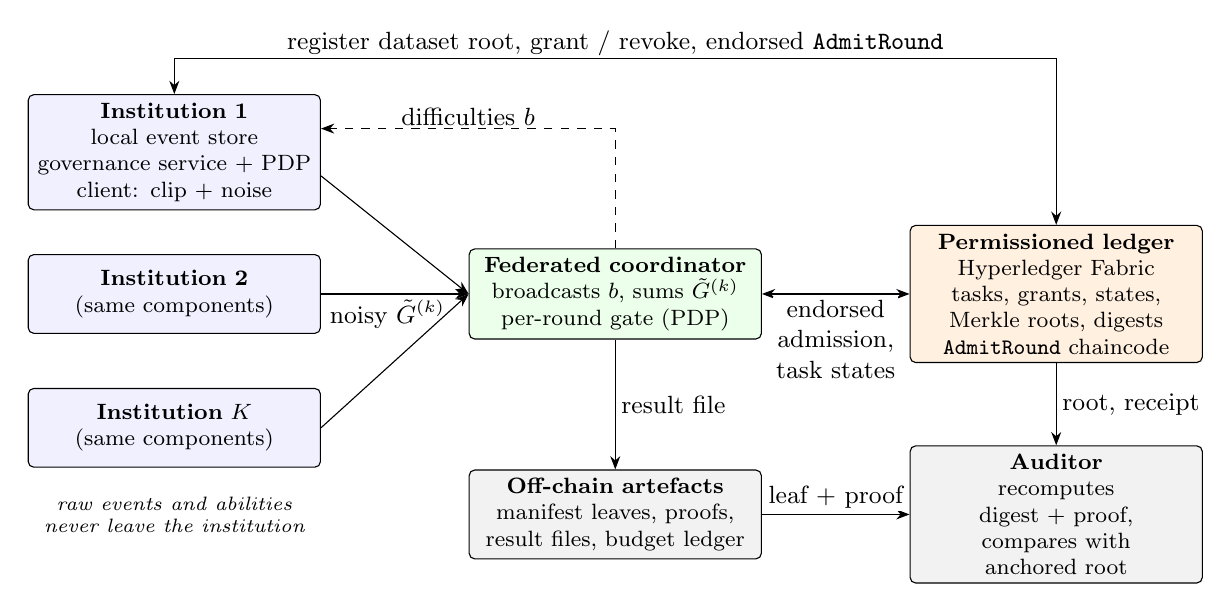
\begin{tikzpicture}[
  font=\footnotesize, >=Stealth,
  box/.style={draw, rounded corners=2pt, align=center, inner sep=3pt, minimum height=1.0cm, text width=3.5cm, execute at begin node={\hyphenpenalty=10000\relax}},
  inst/.style={box, fill=blue!6},
  chain/.style={box, fill=orange!12},
  coord/.style={box, fill=green!8},
  off/.style={box, fill=gray!10},
  lab/.style={font=\small, align=center, fill=white, inner sep=1pt}
]
\node[inst] (i1) at (0,2.6) {\textbf{Institution 1}\\local event store\\governance service + PDP\\client: clip + noise};
\node[inst] (i2) at (0,0.8) {\textbf{Institution 2}\\(same components)};
\node[inst] (ik) at (0,-0.9) {\textbf{Institution $K$}\\(same components)};
\node[coord] (co) at (5.6,0.8) {\textbf{Federated coordinator}\\broadcasts $b$, sums $\tilde G^{(k)}$\\per-round gate (PDP)};
\node[chain] (lg) at (11.2,0.8) {\textbf{Permissioned ledger}\\Hyperledger Fabric\\tasks, grants, states,\\Merkle roots, digests\\\texttt{AdmitRound} chaincode};
\node[off] (oc) at (5.6,-2.0) {\textbf{Off-chain artefacts}\\manifest leaves, proofs,\\result files, budget ledger};
\node[off] (au) at (11.2,-2.0) {\textbf{Auditor}\\recomputes digest + proof,\\compares with anchored root};

\draw[->] ([yshift=-3mm]i1.east) -- (co.west);
\draw[->] (i2.east) -- node[lab, below=1pt, pos=0.45] {noisy $\tilde G^{(k)}$} (co.west);
\draw[->] (ik.east) -- (co.west);
\draw[->, dashed] (co.north) |- node[lab, pos=0.75, above] {difficulties $b$} ([yshift=3mm]i1.east);
\draw[<->] (i1.north) -- ++(0,0.45) -| node[lab, pos=0.25, above] {register dataset root, grant / revoke, endorsed \texttt{AdmitRound}} (lg.north);
\draw[<->] (co.east) -- node[lab, below=1pt] {endorsed\\admission,\\task states} (lg.west);
\draw[->] (co.south) -- node[lab, right=1pt] {result file} (oc.north);
\draw[->] (oc.east) -- node[lab, above=1pt] {leaf + proof} (au.west);
\draw[->] (lg.south) -- node[lab, right=1pt] {root, receipt} (au.north);
\node[font=\scriptsize\itshape, align=center] at (0,-2.0) {raw events and abilities\\never leave the institution};
\end{tikzpicture}}
\caption{Architecture. Raw events, per-student quantities, Merkle leaves and proofs stay off chain; the ledger holds identifiers, codes, states, Merkle roots and receipts. The access predicate is evaluated by each institution's policy decision point and by chaincode}
\label{fig:arch}
\end{widefigure}

Figure~\ref{fig:arch} shows the components. Each institution runs a governance service with the policy decision point (PDP) and a client that computes its round messages locally; a coordinator aggregates rounds; a ledger adapter is the only component that talks to the blockchain. The ledger holds institution and task identifiers, purpose codes, task states, grant records, configuration digests, Merkle roots and result digests. It never holds names, student identifiers or per-student digests, raw answers, per-student vectors or keys.

\subsection{Task-bound purpose enforcement}\label{sec:policy}
A request carries a principal $p$, an action $a$, a task $t$, a resource $r$ of institution $\mathrm{org}(r)$, an output type $o$ and an evaluation time $\tau$; $g$ is the latest grant for $(t,r,\mathrm{org}(r))$. The decision is
\begin{equation}\label{eq:predicate}
\begin{aligned}
\mathrm{allow} \iff\;& \mathrm{valid}(p) \wedge a \in \mathrm{Cap}(p)\\
&\wedge t \text{ exists} \wedge \mathrm{scope}(p,a,r,t)\\
&\wedge a \in \mathrm{Legal}(\mathrm{state}(t)) \\
&\wedge \big(a \in \mathcal{A}_g \Rightarrow g \text{ exists}\\
&\quad\wedge \mathrm{purpose}(g)=\mathrm{purpose}(t)\\
&\quad\wedge \neg\mathrm{revoked}(g)\\
&\quad\wedge \tau < \mathrm{expires}(g)\big) \\
&\wedge \big(a = \texttt{read\_result} \Rightarrow o = \mathrm{output}(t)\\
&\quad\wedge o \in \mathrm{Out}(p)\big),
\end{aligned}
\end{equation}
where $\mathrm{Cap}(p)$ and $\mathrm{Out}(p)$ are those of $p$'s role, the grant-bound actions $\mathcal{A}_g$ are joining, running a round and reading a result, $\mathrm{revoked}(g)$ is a flag in the current state, and $\mathrm{scope}$ requires $\mathrm{org}(p)=\mathrm{org}(r)$ for grant, revoke, join and run actions and $\mathrm{org}(r)$ to participate in $t$ for join and run. $\mathrm{Legal}$ lists the actions each task state permits: \texttt{grant}, \texttt{revoke} and \texttt{read\_audit} in \texttt{draft}; these and \texttt{join\_task} in \texttt{approved}; these and \texttt{run\_round} in \texttt{running}; \texttt{read\_result}, \texttt{revoke} and \texttt{read\_audit} in \texttt{completed}; \texttt{revoke} and \texttt{read\_audit} in \texttt{cancelled}. State changes follow the transition relation of Section~\ref{sec:model}. The conjuncts are evaluated in a fixed order and the first failing one yields a reason code such as \texttt{PURPOSE\_MISMATCH} or \texttt{GRANT\_REVOKED}. The grant names a task, so data cannot be reused by another task with the same purpose; its purpose must equal the task's (A3); and admission is decided for every institution before every round, so expiry or revocation acts at the next round boundary (A2).

\textbf{Dual enforcement.} The chaincode implements the same predicate, order and reason codes over on-chain state. The read-only \texttt{CheckAccess} evaluates it at a caller-chosen time for replay and testing and admits nothing. Admission uses \texttt{AdmitRound}, which an institution's client submits as a transaction under the default majority endorsement policy, and which refuses a caller whose organisation does not own the institution (A7).

\textbf{Evaluation time.} The $\tau$ of \texttt{AdmitRound} is the transaction timestamp. The submitting client writes it into its signed proposal, and neither endorsers nor the ordering service compare it with a clock, so on its own it would let a client choose $\tau$. Each endorser therefore refuses a proposal whose timestamp differs from its clock by more than $\Delta$ ($\Delta=\TsTolerance$~s); the clock decides only acceptance and enters no decision or state. A client can shift $\tau$ by at most $\Delta$, which bounds how far it can stretch an expiry, while revocation denies at any $\tau$. Fabric validates the versions of the task and grant keys that \texttt{AdmitRound} read, so an admission endorsed before a revocation is invalidated if the revocation is ordered first.

\textbf{Audit and writes.} Each admission decision, with its reason code and transaction identifier, is anchored in the next audit batch, so an auditor can check every round gate against the ledger. Grant and revocation writes are accepted only from the organisation that registered the institution (A7), duplicate identifiers are rejected (A6), and tasks start in \texttt{draft}.

\subsection{Provenance anchoring}\label{sec:anchoring}
A dataset version is a manifest of event records, each serialised to a fixed-width byte string and hashed as a Merkle leaf $H(\texttt{0x00}\,\|\,\textit{salt}\,\|\,x)$ with a fresh 128-bit salt per version, kept off chain so that a leaked proof cannot be combined with candidate records. Inner nodes are $H(\texttt{0x01}\,\|\,\ell\,\|\,r)$ with SHA-256, as in Certificate Transparency~\cite{laurie2013certificate}. Audit events and result files are batched the same way. A single artefact is verified by recomputing its digest and combining it with $\lceil\log_2 n\rceil$ sibling hashes up to the anchored root. Table~\ref{tab:chaincode} lists the chaincode interface; a batch of $B$ records costs one transaction instead of $B$.

\begin{table}[t]
\centering
\caption{Chaincode interface}
\label{tab:chaincode}
\footnotesize
\begin{tabular}{@{}p{0.36\columnwidth}p{0.58\columnwidth}@{}}
\toprule
Function & Purpose and checks \\
\midrule
RegisterInstitution & bind an institution to the caller's organisation \\
Register\-Dataset\-Version & manifest root and size; caller owns the institution \\
CreateAnalysisTask, SetTaskState & new tasks start in draft; legal transitions only \\
Grant/Revoke\-Analysis\-Access & task-, resource- and purpose-bound grant with expiry; issuer owns the institution \\
AdmitRound & endorsed admission at the transaction timestamp, within $\Delta$ of the endorser's clock \\
CheckAccess(Batch) & read-only evaluation at a chosen time \\
RecordCalibration, RecordModelVersion & bind a result digest to a completed task and its dataset versions \\
AnchorBatch, VerifyAuditProof & anchor a Merkle root; verify a leaf and proof \\
\bottomrule
\end{tabular}
\end{table}

\section{Federated item calibration}\label{sec:calibration}

The Rasch model~\cite{rasch1960probabilistic} sets $\Pr(y_{ui}=1)=\sigma(\theta_u-b_i)$ for student ability $\theta_u$ and item difficulty $b_i$. We maximise the concave penalised log-likelihood
\begin{equation}\label{eq:obj}
\begin{aligned}
\mathcal{L}={}&\textstyle\sum_{(u,i)}\big[y_{ui}\log\sigma(\theta_u-b_i)\\
&+(1-y_{ui})\log\sigma(b_i-\theta_u)\big]-\tfrac{\lambda}{2}\big(\|\theta\|^2+\|b\|^2\big)
\end{aligned}
\end{equation}
with $\lambda=1$ by alternating diagonal Newton steps~\cite{baker2004item}. With $p_{ui}=\sigma(\theta_u-b_i)$, $G_i=\sum_u (p_{ui}-y_{ui})$ and $H_i=\sum_u p_{ui}(1-p_{ui})$, the ability step uses only $u$'s responses, and the difficulty step is
\begin{equation}\label{eq:bstep}
b_i\leftarrow b_i+\frac{G_i-\lambda b_i}{H_i+\lambda}.
\end{equation}
The pooled procedure is CEN, a reference that needs all raw responses in one place.

\textbf{Exact federated calibration (FED).} Since $G_i=\sum_k G_i^{(k)}$ and $H_i=\sum_k H_i^{(k)}$, the coordinator broadcasts $b$, every admitted institution runs the ability step for its students and returns $(G^{(k)},H^{(k)})$, and the coordinator applies Eq.~\eqref{eq:bstep}. Abilities never leave an institution.

\begin{proposition}\label{prop:exact}
If every institution is admitted in every round and performs one ability step per round, FED and CEN started from the same point produce the same iterates.
\end{proposition}
\begin{proof}
Each ability step uses only the student's own responses, and $G_i,H_i$ are sums over institutions; by induction the iterates agree.
\end{proof}
This follows from additivity over disjoint students and has also been reported by FedIRT~\cite{zhou2025federated}; we state it because the round gate relies on it: excluding an institution changes only which contributions enter $G$ and $H$. Across all our runs the largest difference between FED and CEN difficulties is \FedMaxDiff{}.

\textbf{Differentially private calibration (DP-FED).} Neighbouring datasets differ in all responses of one student. In release~0, each institution scales every student's vector of response and correct counts to L2 norm at most $C_n$ and releases the sums with Gaussian noise $\mathcal{N}(0,\sigma^2C_n^2)$ per coordinate. From the noisy totals $\hat n,\hat c$ the coordinator initialises
\begin{equation}\label{eq:warm}
b_i^{(0)}=-\operatorname{logit}\frac{\hat c_i+m/2}{\hat n_i+m},
\end{equation}
with $m=\max(2,\sqrt{K}\sigma C_n)$, a pseudo-count that shrinks towards $b=0$ when count noise dominates; with no further rounds this is a private count estimator, DP-CNT. In rounds $1..T$, each admitted institution scales each student's gradient contribution $v_u\in\mathbb{R}^I$ to norm at most $C$ and releases $\sum_u \bar v_u+\mathcal{N}(0,\sigma^2C^2 I)$, and the coordinator applies the damped step
\begin{equation}\label{eq:dpstep}
b\leftarrow b+\eta\,\frac{\tilde G-\lambda b}{\tfrac14\hat n+\lambda+\tau},
\end{equation}
where $\tfrac14\hat n$ bounds $H$ from public noisy counts and $\tau=\sqrt{K}\sigma C$, the standard deviation of the aggregated noise, damps steps in proportion to the noise. $T$ is fixed in advance.

\begin{theorem}\label{thm:dp}
The $T+1$ releases of any institution satisfy $\rho$-zCDP with $\rho=(T+1)/(2\sigma^2)$ with respect to adding or removing one student, and hence $(\rho+2\sqrt{\rho\ln(1/\delta)},\delta)$-differential privacy.
\end{theorem}
\begin{proof}
Each release is a Gaussian mechanism with the clipping norm as sensitivity (other students' abilities depend only on their own responses and the released $b$), hence $1/(2\sigma^2)$-zCDP~\cite{bun2016concentrated}; zCDP composes additively, and the coordinator only post-processes.
\end{proof}

Given $(\varepsilon,\delta)$ we solve for $\rho$ and set $\sigma=\sqrt{(T+1)/(2\rho)}$; tighter conversions exist~\cite{canonne2020discrete}, but the protocol fixed this one. Each institution adds its own noise, so the guarantee does not depend on the coordinator; with secure aggregation~\cite{bonawitz2017practical} the same guarantee would need $\sqrt{K}$ times less total noise (Section~\ref{sec:eval-privacy}). Each institution's \emph{budget ledger} charges all $T+1$ releases before a task starts and refuses the task if the remaining budget is insufficient; an institution excluded by the round gate releases nothing further.

\section{Implementation}\label{sec:impl}

The prototype has a Python package (policy engine, Merkle trees, zCDP accountant and budget ledger, calibration), JavaScript chaincode and a Node.js bridge on the Fabric Gateway SDK. The network is the Fabric \FabricVersion{} test network: two organisations with one peer each, one Raft orderer, TLS, majority endorsement and default block cutting (\FabricBatchTimeout{} batch timeout, at most \FabricMaxMsg{} transactions per block), with chaincode run as an external service. The utility and privacy experiments ran offline, because with every institution admitted the gate changes nothing in the arithmetic; the gated path is measured end to end in Section~\ref{sec:eval-access}.

\section{Evaluation}\label{sec:eval}

We ask: Q1, how close is FED to CEN on non-IID institutions and what do simpler alternatives lose; Q2, what does student-level differential privacy cost; Q3, does enforcement stop what it should, and do backend and chaincode agree; Q4, what does anchoring cost?

\subsection{Setup}\label{sec:setup}
The main experiments follow a protocol that fixed datasets, partitions, methods, metrics, selection rules and repetitions before any run; later analyses are marked exploratory. One departure occurred: the first DP-FED version diverged during hyper-parameter selection on synthetic data and was replaced, before any real-data run, by the estimator of Section~\ref{sec:calibration}. Hyper-parameters were selected on synthetic data only and frozen: $T=\HpT$, $C=\HpC$, $C_n=\HpCn$, $\eta=\HpLr$, $\lambda=1$, $\delta=10^{-5}$. FED and CEN stop when the largest update falls below $10^{-6}$ (at most 500 rounds).

\textbf{Data.} \emph{ASSISTments 2009--2010}~\cite{feng2009addressing}: original problems, the \AssistNSchools{} schools with at least 5{,}000 responses as institutions, items with at least 20 responses and students with at least 5 (\AssistUsers{} students, \AssistItems{} items, \AssistResp{} responses). \emph{Junyi Academy}~\cite{junyi2020dataset,chang2015modeling}: the \JunyiNCities{} cities with most attempts as institutions, items with at least 50 attempts and students with at least 10 (\JunyiUsers{} students, \JunyiItems{} items, \JunyiResp{} attempts); a city is a coarse proxy for an institution. \emph{Synthetic} Rasch data: 500 items with $b_i\sim\mathcal{N}(0,1)$, $K\in\{3,10\}$ institutions of 300 students answering 40 items; in the non-IID regime mean abilities span $[-1,1]$ and each institution draws from its own window of 250 items. The item thresholds depend on pooled counts and so fall outside Theorem~\ref{thm:dp}; we treat them as a convenience of this evaluation, and a deployment calibrates the public catalogue or thresholds the noisy counts of release~0, which is post-processing. So is the choice of the largest schools or cities.

\textbf{Metrics.} We report test AUC of $\sigma(\hat\theta_u-\hat b_i)$, and the RMSE and Spearman correlation (average ranks) of centred difficulties against the truth (synthetic) or CEN (real). CNT is the centred logit of each item's pooled smoothed success rate; LOC fits the Rasch model within each institution, leaving unseen items at $b=0$. Each configuration uses \NSeeds{} seeds, which change each student's 80/20 split of responses into training and test and, for DP, the noise. Calibration ran single-threaded on one laptop (\HostCPU{}, \HostRAM{}~GB). The access-control timings of Section~\ref{sec:eval-access} were taken while unrelated jobs loaded this host (load average about 13 on 8 hardware threads), so their processing times are pessimistic.

\subsection{Q1: utility without privacy}\label{sec:eval-utility}

\begin{widetable}
\centering
\caption{Real multi-institution logs: test-set prediction and agreement with the centralised reference, mean over seeds ($\pm$ s.d. for AUC).}
\label{tab:real}
\small
\begin{tabular}{llcccc}
\toprule
Dataset & Method & AUC & Brier & b-RMSE & Spearman $\rho$ \\
\midrule
ASSIST09 & CEN & 0.7580$\pm$0.0022 & 0.1836 & 0.000 & 1.000 \\
 & LOC & 0.7481$\pm$0.0032 & 0.1867 & 0.726 & 0.376 \\
 & CNT & 0.7472$\pm$0.0031 & 0.1870 & 0.343 & 0.916 \\
 & FED & 0.7580$\pm$0.0022 & 0.1836 & 0.000 & 1.000 \\
\midrule
Junyi & CEN & 0.7507$\pm$0.0002 & 0.1714 & 0.000 & 1.000 \\
 & LOC & 0.7513$\pm$0.0003 & 0.1712 & 0.271 & 0.938 \\
 & CNT & 0.7482$\pm$0.0003 & 0.1721 & 0.272 & 0.953 \\
 & FED & 0.7507$\pm$0.0002 & 0.1714 & 0.000 & 1.000 \\
\bottomrule
\end{tabular}
\par\smallskip\footnotesize b-RMSE and $\rho$ are measured against CEN, which is a reference, not ground truth; CEN and FED therefore show 0 and 1.
\end{widetable}

FED reproduces CEN in every run (Table~\ref{tab:real} for the real logs). On synthetic data with IID institutions CNT is close to FED (RMSE \SynTenIidCNTRmse{} against \SynTenIidFEDRmse{}, $K=10$); in the non-IID regime it rises to \SynTenNonCNTRmse{} against \SynTenNonFEDRmse{}, because a pooled success rate attributes the ability of an item's students to the item. On ASSISTments, CNT and LOC reach lower AUC (\AssistCNTAuc{}, \AssistLOCAuc{}) than FED (\AssistFEDAuc{}); the median school saw only \AssistCovMedian\% of the items. On Junyi, with about \JunyiRespPerItem{} training attempts per item, CNT reaches \JunyiCNTAuc{} and LOC \JunyiLOCAuc{}, slightly above FED (\JunyiFEDAuc{}); across seeds FED differs from LOC by \GJunyiFedLocDiff{} AUC.

\textbf{Where a shared scale pays off (exploratory).} Abilities are always fitted on the predicted institution's training responses. (a) On synthetic non-IID data, difficulties fitted on the other nine institutions predict a held-out institution with AUC \GSynFedAuc{} (FED) against \GSynLocAuc{} (its own LOC fit) and \GSynCntAuc{} (CNT); FED wins \GSynFedWins{} of \GSynLOON{} pairs (Wilcoxon $p=\GSynFedLocP$). (b) When 20\% of an institution's items are withheld from its own training only, FED predicts responses on them with AUC \GUnseenFedAuc{} and RMSE \GUnseenFedRmse{}, against \GUnseenLocAuc{} and \GUnseenLocRmse{} for LOC and \GUnseenCntAuc{} and \GUnseenCntRmse{} for CNT (FED beats LOC in \GUnseenFedWins{} of \GUnseenN{} pairs). (c) On Junyi, with each FED fit started from zero so that nothing of the held-out city enters it (\GLooSeeds{} seeds, \GLooCities{} cities), FED trails LOC by \GLooFedLocDiff{} AUC (95\% cluster-bootstrap interval \GLooFedLocLo{} to \GLooFedLocHi{}) and leads CNT by \GLooFedCntDiff{} (\GLooFedCntLo{} to \GLooFedCntHi{}). A shared scale thus costs little when institutions can calibrate alone, helps when they cannot, and supplies difficulties for items an institution has not seen.

\subsection{Q2: the cost of differential privacy}\label{sec:eval-privacy}

\begin{widefigure}
\centering
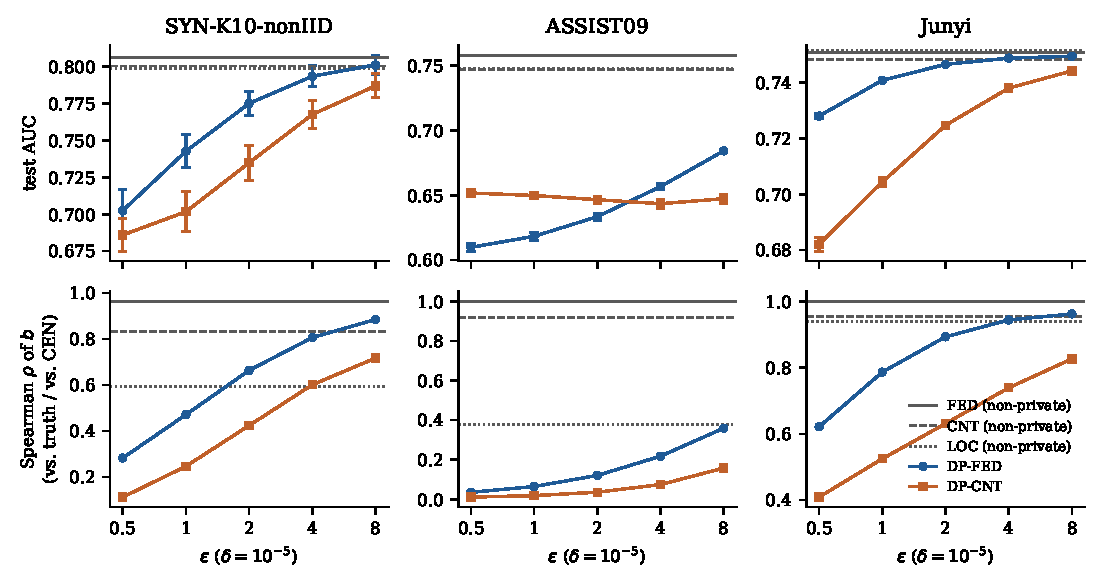
\includegraphics[width=0.66\textwidth]{figures/privacy_utility.pdf}
\caption{Privacy--utility trade-off of DP-FED ($T=\HpT$) and DP-CNT, mean over seeds. Top: test AUC (error bars: s.d.). Bottom: Spearman correlation of private difficulties with the truth (synthetic) or CEN (real). Horizontal lines: non-private FED, CNT and LOC}
\label{fig:privacy}
\end{widefigure}

All private runs satisfy Theorem~\ref{thm:dp}. The cost depends on the data behind each release (Fig.~\ref{fig:privacy}). On Junyi (\JunyiUsers{} students), DP-FED at $\varepsilon=2$ reaches AUC \JunyiDPFEDTwoAuc{} against \JunyiFEDAuc{} non-privately, with Spearman $\rho=\JunyiDPFEDTwoRho{}$ to CEN. On ASSISTments (\AssistUsers{} students, about \AssistRespPerItem{} attempts per item) it reaches only \AssistDPFEDTwoAuc{} against \AssistFEDAuc{}, with $\rho=\AssistDPFEDTwoRho{}$, and even at $\varepsilon=8$ the rank agreement is \AssistDPFEDEightRho{}. On Junyi and non-IID synthetic data DP-FED beats DP-CNT at every $\varepsilon$ although it spends its budget on $T+1$ releases.

\begin{widetable}
\centering
\caption{Trusted-aggregator baseline versus DP-FED (exploratory). The baseline adds one noise draw of standard deviation $\sigma C$ per round to the aggregated gradient, and likewise for the counts, that is $\sqrt{K}$ times less total noise than per-institution releases at the same $(\varepsilon,\delta)$. The factor is DP-FED RMSE divided by baseline RMSE. AUC uses the same evaluation as Table~\ref{tab:real}. Mean over \NSeeds{} seeds on synthetic non-IID data with $K=10$ and \ExSeedsJunyi{} seeds on Junyi.}
\label{tab:fedirtdp}
\footnotesize\setlength{\tabcolsep}{4pt}
\begin{tabular}{l rrr rr rrr rr}
\toprule
& \multicolumn{5}{c}{Synthetic non-IID, $K=10$} & \multicolumn{5}{c}{Junyi} \\
\cmidrule(lr){2-6}\cmidrule(lr){7-11}
$\varepsilon$ & \multicolumn{2}{c}{RMSE} & factor & \multicolumn{2}{c}{AUC} & \multicolumn{2}{c}{RMSE} & factor & \multicolumn{2}{c}{AUC} \\
& DP-FED & baseline & & DP-FED & baseline & DP-FED & baseline & & DP-FED & baseline \\
\midrule
0.5 & 1.446 & 0.957 & 1.51 & 0.7024 & 0.7670 & 0.812 & 0.438 & 1.85 & 0.7280 & 0.7454 \\
1 & 1.148 & 0.693 & 1.66 & 0.7426 & 0.7895 & 0.573 & 0.302 & 1.90 & 0.7407 & 0.7484 \\
2 & 0.861 & 0.509 & 1.69 & 0.7750 & 0.8003 & 0.392 & 0.233 & 1.69 & 0.7465 & 0.7493 \\
4 & 0.634 & 0.411 & 1.54 & 0.7934 & 0.8039 & 0.281 & 0.211 & 1.33 & 0.7487 & 0.7496 \\
8 & 0.489 & 0.372 & 1.32 & 0.8010 & 0.8049 & 0.230 & 0.206 & 1.12 & 0.7494 & 0.7496 \\
\bottomrule
\end{tabular}
\end{widetable}

\textbf{Trusted-aggregator baseline (exploratory).} FedIRT-DP~\cite{zhou2025federated} adds noise once, at a trusted aggregator, which needs $\sqrt{K}$ times less total noise than our per-institution releases. Running our estimator with that noise pattern, the same splits and noise seeds (Table~\ref{tab:fedirtdp}) shows that DP-FED's difficulty RMSE is \ExRatioMin{} to \ExRatioMax{} times the baseline's, narrowing at large $\varepsilon$; on Junyi at $\varepsilon=2$ it is \ExJunyiFedTwoRmse{} against \ExJunyiSecTwoRmse{}, with AUC \ExJunyiFedTwoAuc{} against \ExJunyiSecTwoAuc{}. This error is the price of a guarantee that does not rely on the coordinator.

\textbf{Damping, clipping and coarser units (exploratory).} Without noise-scaled damping, Junyi RMSE at $\varepsilon=2$ grows from \AblJunyiFullTwoRmse{} to \AblJunyiNoDampTwoRmse{}; without the pseudo-count, AUC at $\varepsilon=1$ falls from \AblJunyiFullOneAuc{} to \AblJunyiNoPseudoOneAuc{}. The frozen clipping norms clip almost every student (\FJunyiClipCntFourPct\% at $C_n$ and \FJunyiGradClipHalfPct\% at $C$ on Junyi), so they act as a normalisation; over a $4\times3$ grid of norms at $\varepsilon=2$, Junyi RMSE ranges from \FJunyiSensRmseMin{} to \FJunyiSensRmseMax{} with the frozen pair at \FJunyiSensFrozenRmse{}. Calibrating ASSISTments per skill (\HSkills{} units) raises DP-FED AUC at $\varepsilon=2$ from \AssistDPFEDTwoAuc{} to \HDpTwoAuc{} against a skill-level ceiling of \HCenAuc{}, but rank agreement stays at \HDpTwoRho{}.

\subsection{Q3: access control on the ledger}\label{sec:eval-access}

\textbf{Agreement of backend and chaincode (C1).} Over \COneTasks{} tasks in all states and \COneGrants{} grants (\COneRevoked{} revoked), created through chaincode and mirrored in the backend, the two implementations returned the same decision, reason code and grant for \COneAgree\% of \COneN{} random requests and \COneBndAgree\% of \COneBndN{} boundary requests at one second before, at and after every expiry and revocation instant (\COneBndAllow{} allowed, \COneBndExpired{} expired, \COneBndRevoked{} revoked, \COneBndPurpose{} purpose mismatch). All \COneNegN{} forbidden writes (foreign organisation, replayed identifiers, illegal transitions, malformed digests) were rejected. A backend decision takes \COnePdpUs{}~$\mu$s and a \texttt{CheckAccess} query \COneChainSingleMs{}~ms at the median. A revocation submitted through one organisation took effect on the other organisation's peer after \RevokeMean{}~s on average, close to the commit time, which is set by the batch timeout.

\textbf{Enforcement points (C2).} In \CTwoTasks{} simulated tasks with \CTwoEvents{} mid-task revocations or expiries, role-only checks admitted \CTwoViolLogin{} unauthorised round participations and join-time checks \CTwoViolJoin{}, while per-round re-evaluation admitted \CTwoViolRound{}. For the weaker points this follows from their definitions.

\begin{table}[t]
\centering
\caption{End-to-end revocation, one run ($K=10$, $T=\EtoeRounds$, revocation before round \EtoeExampleRound{}); RMSE against true difficulties}
\label{tab:etoe}
\footnotesize
\begin{tabular}{@{}p{0.72\columnwidth}r@{}}
\toprule
Revocation, submission to commit & \EtoeExampleCommit{}~s \\
First round without the institution & \EtoeExampleExcluded{} \\
Anchored admission records (denials) & \EtoeExampleRecords{} (\EtoeExampleDenied{}) \\
FED RMSE, uninterrupted $\to$ revoked & \EtoeExampleFedBefore{} $\to$ \EtoeExampleFedAfter{} \\
DP-FED RMSE, uninterrupted $\to$ revoked & \EtoeExampleDpBefore{} $\to$ \EtoeExampleDpAfter{} \\
\bottomrule
\end{tabular}
\end{table}

\textbf{End-to-end revocation (C2-E2E).} We ran DP-FED (non-IID synthetic data, $K=10$, $\varepsilon=2$) on the deployed network with every round gated by concurrent \texttt{AdmitRound} transactions, revoking one grant before round \EtoeRevokeRounds{} in \EtoeRuns{} runs. In every run the institution was excluded from the first round after the commit (Table~\ref{tab:etoe}); commits took \EtoeCommitMean{}~s on average. When the revocation was submitted concurrently with the admissions of round \EtoeRaceRound{}, the institution's admission \EtoeRaceReason{} and it was excluded from that round. An auditor using only the anchored admission logs and the ledger verified \EtoeAuditProofs{} of \EtoeAuditRecords{} records, found all transactions valid with matching block and time, and reproduced \EtoeAuditDecisions{} decisions by evaluating Eq.~\eqref{eq:predicate} at the logged times. Earlier releases stay in the estimate, so the result changes little; the DP-FED pair also differs in noise. Gating costs latency rather than throughput: a gate took \EtoeGateBefore{}~s while ten admissions filled a block and \EtoeGateAfter{}~s afterwards, adding \EtoeGateTotal{}~s per task against \EtoeOffline{}~s of computation; with $K=3$ every gate waited for the batch timeout (\EtoeThreeGate{}~s). Proposals with forged timestamps were evaluated at the forged time up to $\pm\TsAcceptedMax$~s and refused from $\pm\TsRejectedMin$~s on.

\textbf{Tamper detection (C3).} All \CThreeClean{} anchored artefacts verified, and all \CThreeDetected{} copies with one flipped bit failed.

\subsection{Q4: anchoring cost}\label{sec:eval-ledger}

\begin{figure}[t]
\centering
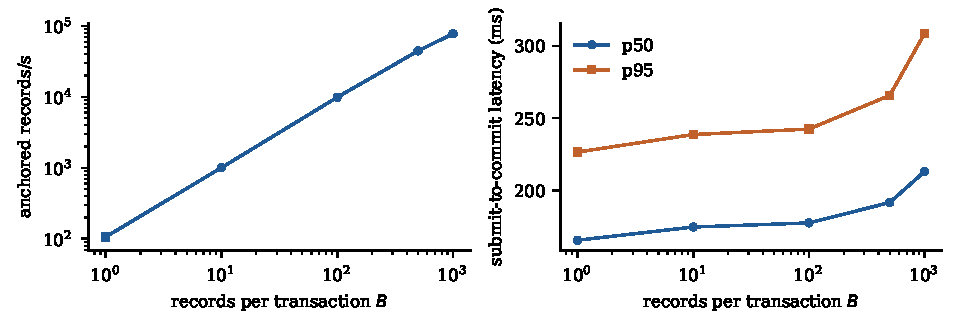
\includegraphics[width=\columnwidth]{figures/anchoring.pdf}
\caption{Anchored records per second (left, log--log) and submit-to-commit latency (right) against batch size $B$; error bars: s.d. over repetitions}
\label{fig:anchoring}
\end{figure}

With \BenchConc{} concurrent clients on an otherwise idle host, the transaction rate stayed between \BenchThousandTx{} and \BenchRecTx{} per second for all batch sizes, so anchored records per second grew from \BenchRecRec{} to \BenchThousandRec{} at $B=1000$ (Fig.~\ref{fig:anchoring}), while median latency rose from \BenchRecPFifty{} to \BenchThousandPFifty{}~ms. A transaction occupied about \BenchRecBpt{} bytes regardless of $B$, so ledger cost follows the number of transactions. Over all \ManN{} Junyi records, salted Merkle trees took \ManLeafSec{}~s to hash and \ManTreeSec{}~s to build; a proof in the largest institution has \ManDepth{} hashes and verifies in about \ManVerifyUs{}~$\mu$s. One Junyi task writes about 25 transactions for ten institutions, whereas its FED messages total about \JunyiFEDBytesMB{}~MiB, which systems that place updates on chain would have to carry. These figures characterise strategies on our small network, not production capacity.

\section{Discussion and limitations}\label{sec:discussion}

The ledger provides governance, not calibration: a shared record of grants, states and digests, and an endorsed evaluation of the predicate, so that no single operator decides whether a round was allowed. Privacy at single-digit $\varepsilon$ is affordable with tens of thousands of students and not with a few thousand, which a consortium can anticipate from public quantities before releasing anything; secure aggregation would remove the $\sqrt{K}$ noise factor. The limitations are as follows. The network ran on one host with two organisations and default settings, and more endorsing organisations would raise latency. Principal attributes come from the institution's service rather than X.509 certificates, a client can shift the evaluation time by up to $\Delta$, and that bound relies on honest clocks. Hyper-parameters were frozen on synthetic data. Cities and the schools of one platform stand in for independent institutions, and the end-to-end run used synthetic data on a shared host. The ledger proves that registered artefacts are unchanged, not that the data were collected correctly.

\section{Conclusion}\label{sec:conclusion}

LearnFlow-Chain treats cross-institution calibration as a governed computation: data and abilities stay local, every round is admitted by an endorsed, purpose- and task-bound predicate that a policy engine and chaincode evaluate identically, and the lineage of every published difficulty is anchored as digests. Exact federated calibration matters most when institutions differ, student-level privacy is affordable at large scale only, and on a deployed network a revoked institution was excluded from the next round and every admission decision could be replayed from the ledger. Secure aggregation, certificate-based attributes and deployment across independent operators are the next steps.

\section*{Declarations}

\textbf{Funding.} To be completed by the authors.

\textbf{Competing interests.} To be completed by the authors.

\textbf{Ethics approval and consent.} Both real datasets are public, de-identified learning logs used under their research-use terms; no data were collected from students and no re-identification was attempted. The synthetic data describe no real persons.

\textbf{Data availability.} ASSISTments 2009--2010~\cite{feng2009addressing} and the Junyi Academy log~\cite{junyi2020dataset} are publicly available from their providers and are not redistributed.

\textbf{Code availability.} To be completed by the authors.

\textbf{Use of AI tools.} To be completed by the authors.

\bibliography{references}

\end{document}